\subsection*{A4O3.2}
To use Prolog to find all the dictionaries that can be passed to \texttt{qsort'} in the different cases, I add the following facts to implement the needed type in the program.

\begin{verbatim}
isTypeOf(list(A),list(A)).

isTypeOf(true,bool).
isTypeOf(false,bool).

isTypeOf(int,int).
\end{verbatim}

Now lets determine the number of dictionaries that can be passed to \texttt{qsort'} by running the quries seen in figure \ref{fig:dicts}.

\begin{figure}[h]
\centering
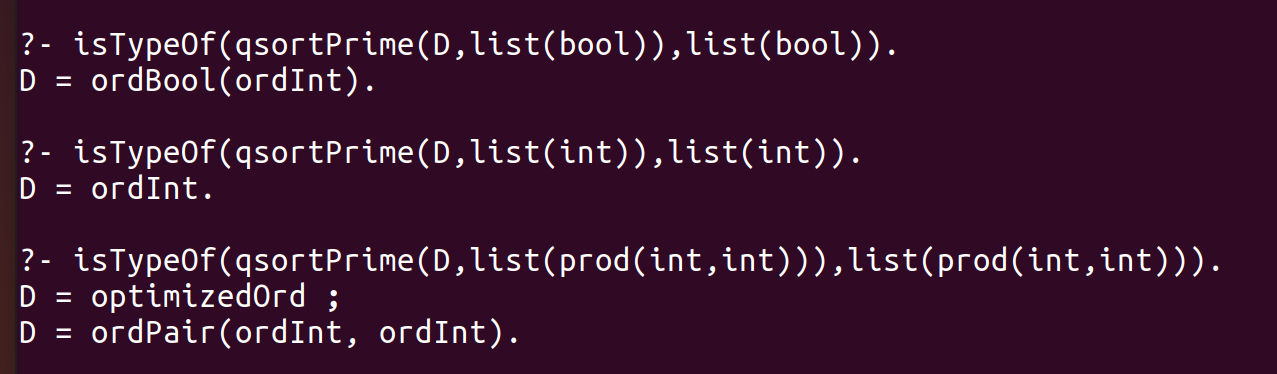
\includegraphics[width=0.8\textwidth]{O32.png}
\caption{Finding dictionaries to be passed to \texttt{qsort'}.}
\label{fig:dicts}
\end{figure}
\newpage
Thus there is one dictionary for boolean lists, one for integer lists, and two for lists of pairs of integers.

Now lets look at the resolution tree for the last query. By using the \textit{trace} command in SWI-Prolog, we can determine the way the program issues the query. This is seen in figure \ref{fig:resTrace}.

\begin{figure}[h]
\centering
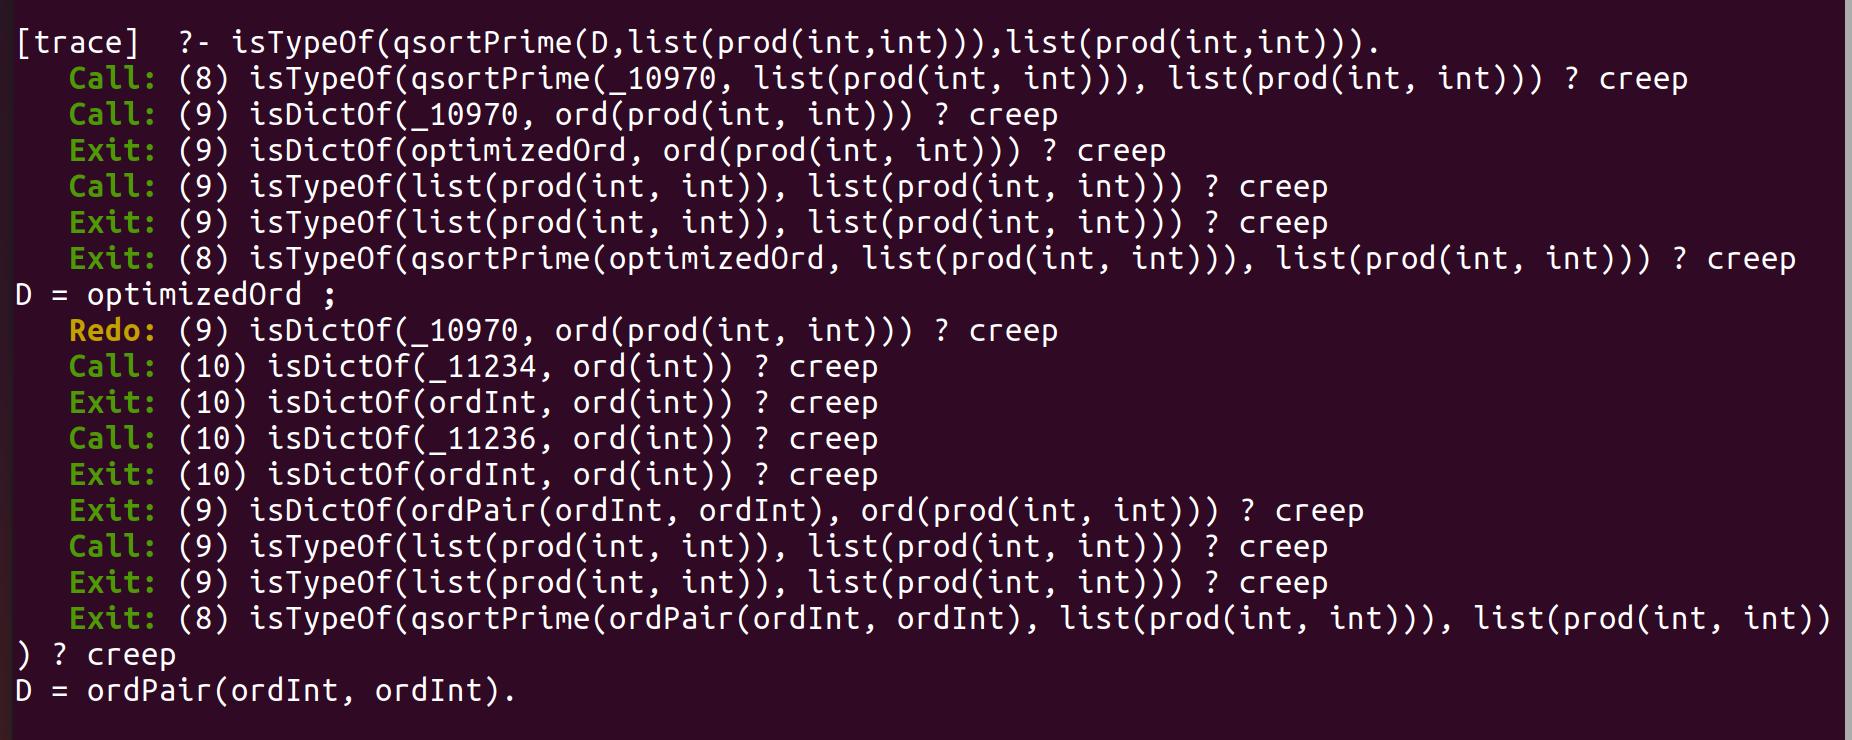
\includegraphics[width=0.8\textwidth]{resTrace.png}
\caption{The result of running the query while \textit{trace} is active.}
\label{fig:resTrace}
\end{figure}

From this the resolution tree shown in figure \ref{fig:resTree} is drawn.

\begin{figure}[h]
\centering
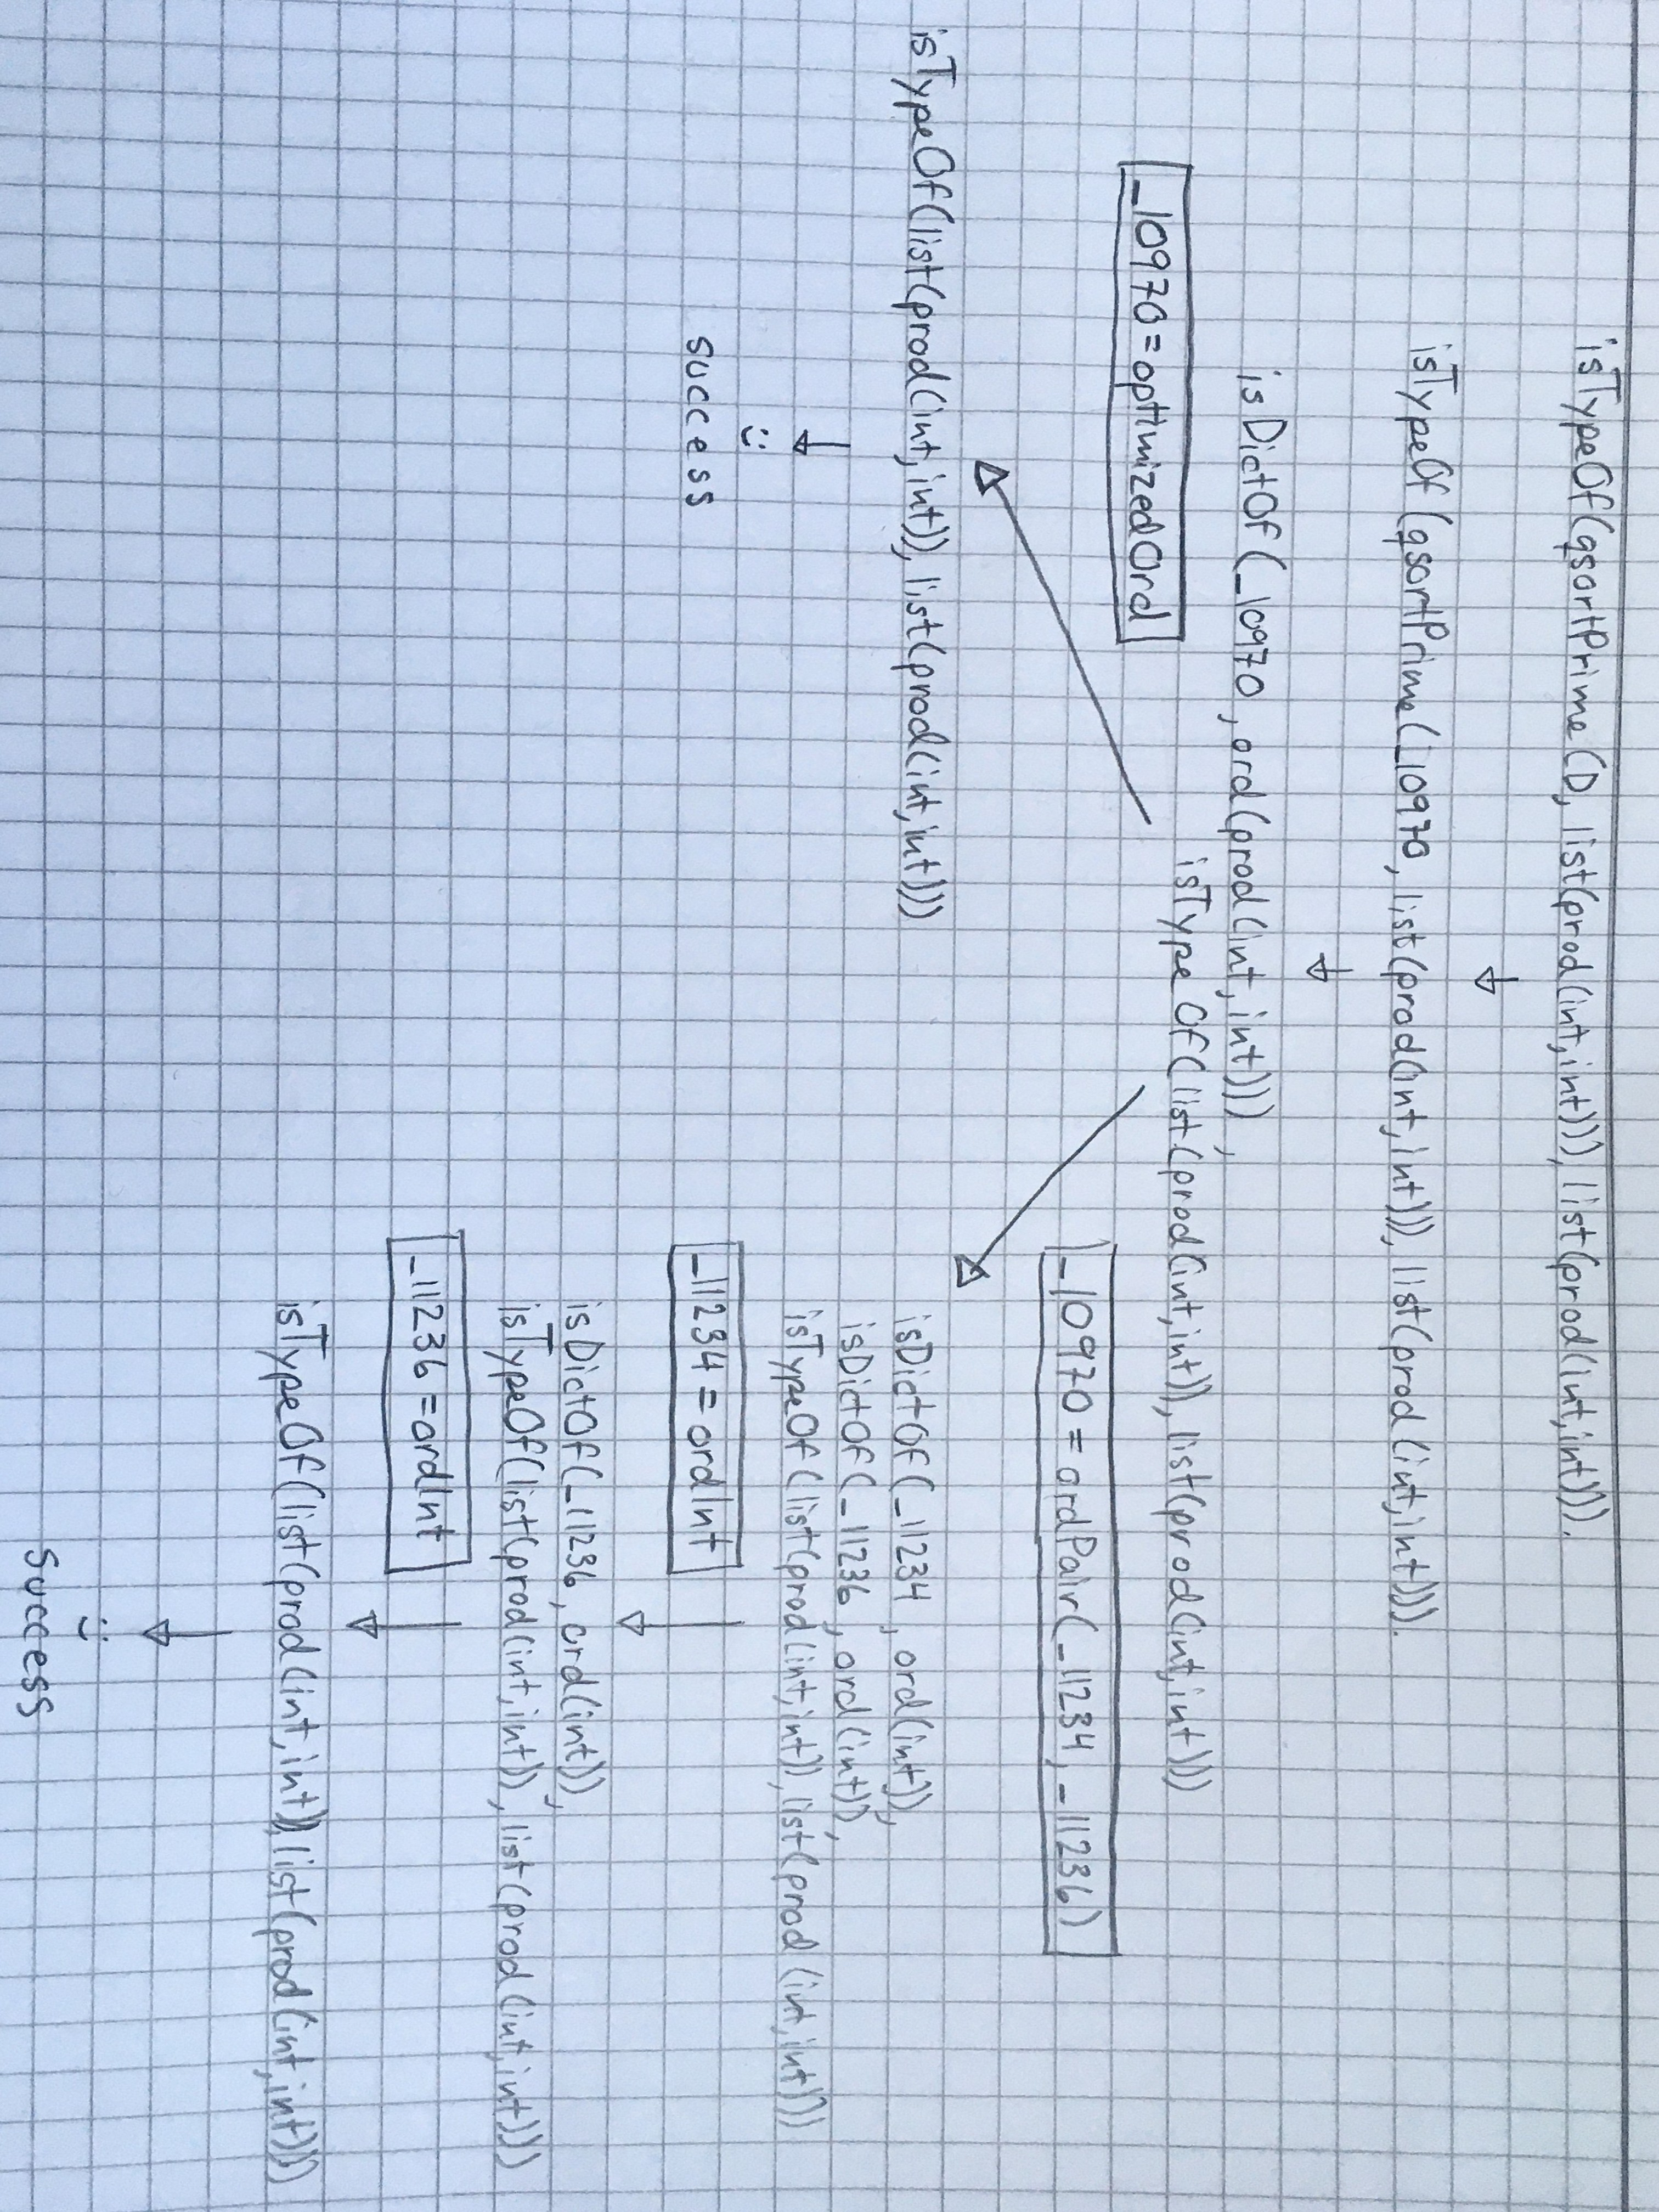
\includegraphics[width=0.8\textwidth]{resTree.jpg}
\caption{The resolution tree for the query.}
\label{fig:resTree}
\end{figure}
